\chapter{Generative and Performative Algorithms}

\section{Introduction}

Today, two main paradigms of algorithmic design are clearly dominant; generative design and performative design \cite{fasoulaki08}. Generative design is the essential \emph{rule-based\footnote{Consisting of a solid set of consecutive instructions that govern an action to produce a desired outcome}} algorithmic form of algorithmic architecture. It is governed by repetitive patterns, equations and shape transformations.  Performative design on the other hand, is optimisational; modifying and reshaping to adapt to a certain simulated environment.

\section{Generative Algorithm}

Generative architecture can be defined as a design process involving generative systems in the form of a computer program that can be fully automated or step-by-step controlled. It would have an algorithm (rule) governing the transformations of initial shapes through variables or parameters; `generating' results, and selecting the best variant according to the given criteria. \cite{arida04}

The tools and key components of generative design are the systems which define the method of form exploration. They can be defined as scripts or sets of geometrical transformations \cite{arida04}. These systems ---as mentioned earlier--- are rule based, essentially formal or visual and are often based on systems borrowed from biology and mathematics. Some popular systems widely used today include Cellular Automata, L-Systems, Voronoi Diagrams, Fractals and Shape Grammars.

\subsection{Cellular Automata}

``Cellular Automata is a computational method which can simulate the process of growth by describing a complex system by simple individuals following simple rules. The concept of simulating growth was introduced by John von Neumann (1951) and further developed by Ulam (1962) in the are of simulating multi-state machines. The concept gained great popularity when Martin Gardner (1970) John Conway's ``Life'', a game that generated two dimensional patterns''\cite{krawczyk02}. Later on, Stephen Wolfram would begin research on the subject in 1984, to write a book on the subject called \emph{A New Kind of Science} \cite{wolfram02}. The book would discuss the patterns created by cellular automata as simple rules capable of generating extremely complex patterns that mimic patterns of growth occurring in nature, among other things; describing his findings as a new paradigm of scientific research touching on numerous fields of science.

\begin{figure}[htbp]
\centering
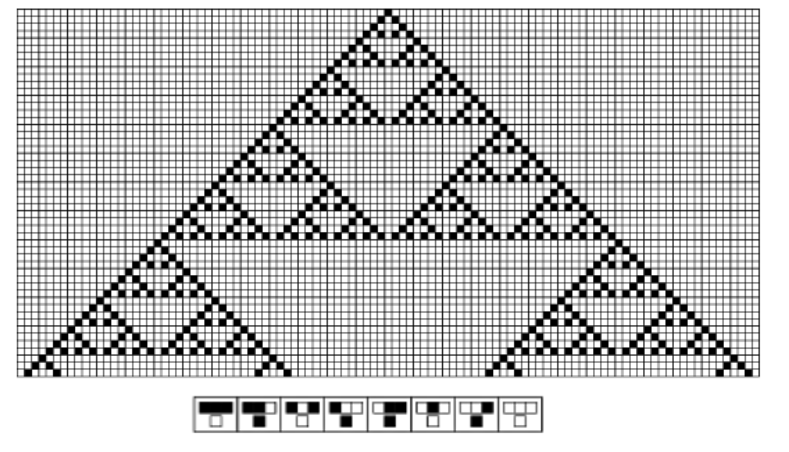
\includegraphics[width=\textwidth]{./Images/1-CellAutoEg}
\caption[Cellular Automaton]{An example of cellular automata showing (a) the sequence of generations and (b) the governing rule.\cite{wolfram02}}
\label{CAEg}
\end{figure}

The concept of cellular automata is that an initial configuration of at least one cell occupying an empty space would evolve and procreate into a pattern using a rule that decides birth, life and death cells through the preceding related cells (Fig. \ref{CAEg}). The pattern shown is a two dimensional growth pattern used by Stephen Wolfram. Other forms of cellular automata generation include 3-dimensional ones, which are the architects main interest.

The method of generation in 3-dimensional cellular automata remains basically the same as with 2-dimensional ones; with an initial configuration of blocks occupying spaces and a rule that governs the shape of each generation (Fig \ref{3dCA}).

\begin{figure}[htbp]
\centering
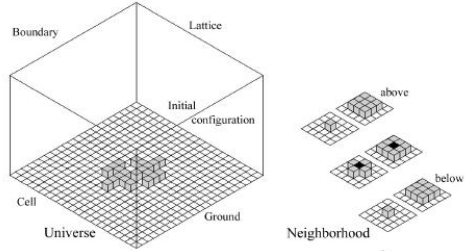
\includegraphics[width=0.7\textwidth]{./Images/2-3dCA}
\caption[3-Dimensional Cellular Automata]{3-Dimensional cellular automata and terminology.\cite{krawczyk02}}
\label{3dCA}
\end{figure}

The utilisation of basic rules of cellular automata however does not suffice to produce architecturally sound models with appropriate internal spaces in most cases (Fig \ref{3dCAArch}). In order to produce such forms, a degree of optimisation and modification is required. A fairly simple but effective solution is manipulation of cell interpretation. Examples of such manipulation are stretching cells to overlap forming adequate internal spaces, merging the overlapping cells and interpreting the envelope of merged cells as splines (Fig \ref{CA Optimisation}).

\begin{figure}[htbp]
\centering
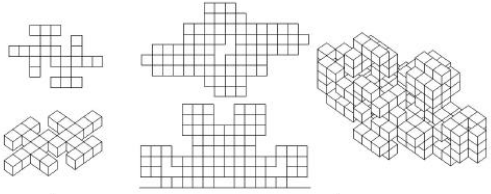
\includegraphics[width=0.7\textwidth]{./Images/3-3dCAArch}
\caption[Cellular Automata Architectural Inadequacy]{An example of CA rules inadequacy for architectural forms without modification \cite{krawczyk02}}
\label{3dCAArch}
\end{figure}


\begin{figure}[htbp]
\centering
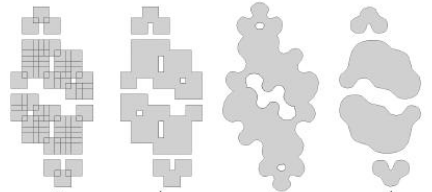
\includegraphics[width=0.7\textwidth]{./Images/4-3dCAArchOpt}
\caption[Cellular Automata Architectural Optimisation]{Optimisation of cell interpretation for architectural form \cite{krawczyk02}}
\label{CA Optimisation}
\end{figure}

Multiple interpretations of the manipulated generations (Fig \ref{CA ArchForm}) were created with structural support. The architectural forms shown appear more developed, nevertheless; it was subject to several modifications of the original cellular automata model which required user intervention at early stages of the process, which would prove CA to be a rather raw method of architectural form generation.

\begin{figure}[H]
\centering
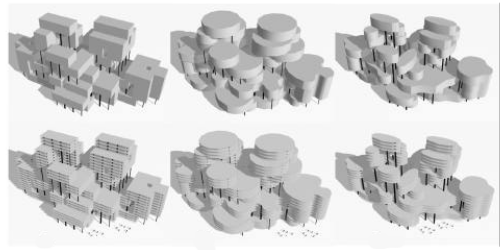
\includegraphics[width=\textwidth]{./Images/5-3dCASpaces}
\caption[Architectural Interpretation of CA Generations]{Architectural Interpretation of CA Generations \cite{krawczyk02}}
\label{CA ArchForm}
\end{figure}

\subsection{Voronoi Diagrams}

``Considered as early as 1644 by Ren\'{e} Descartes but are named after the Russian Mathematician Georgy Fedoseevich Voronoi who studied and defined the general n-dimensional case in 1907''\cite{fasoulaki08}. A Voronoi Diagram is a way of decomposing a space into regions\footnote{Voronoi Diagrams are a class of patterns called Dirichlet tessellations}, this process initiate with a set of points in space; called generating points, the partitioning lines are then drawn from an equal distance from the aforementioned points creating polygons or cells (Fig. \ref{VDiag}).

\begin{figure}[htbp]
\centering
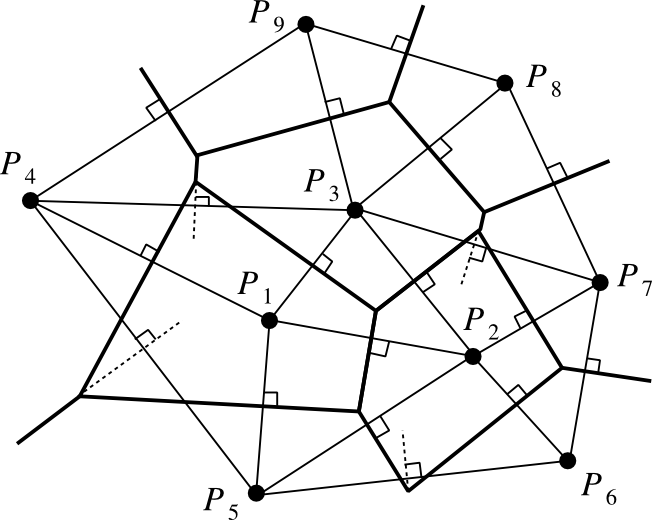
\includegraphics[width=0.8\textwidth]{./Images/6-VoronoiDiagram}
\caption[Voronoi Diagram]{Voronoi Diagram \cite{fujita00}}
\label{VDiag}
\end{figure}

Voronoi Diagrams are naturally occurring patterns such as crystalline formations, bee honeycombs and animal coat patterns among other things, making it a suitable model of form generation and optimisation as well in terms of structure \cite{friedrich08} and environmental performance\label{NaturalOpt}. The main form of utilisation however is that of internal space division or partitioning (Fig. \ref{VDInternal}) and urban design and planning (Fig. \ref{VDUrban})

Although the common form of utilisation of Voronoi Diagram might denote a 2-dimensional constraint, it is also used in 3-dimensional space generating surfaces points in 3D space.

\begin{figure}[htbp]
\centering
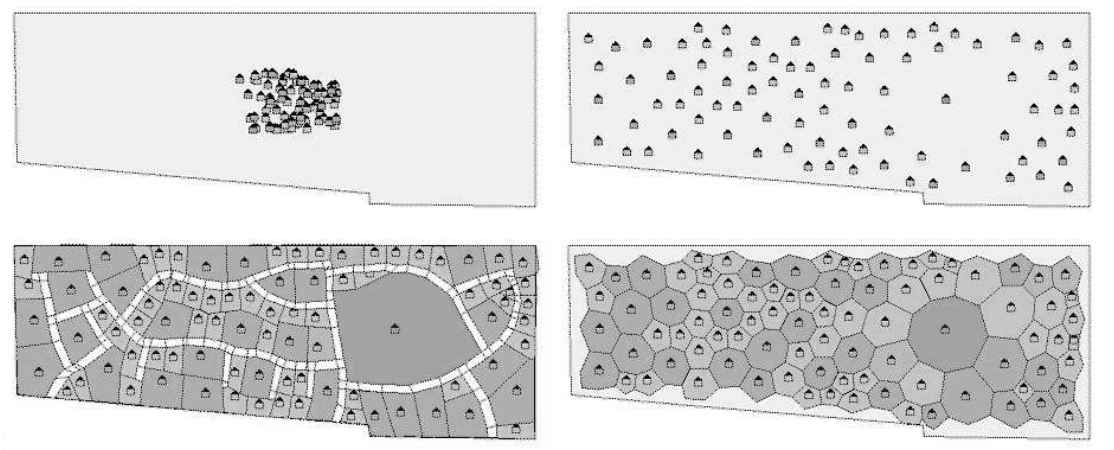
\includegraphics[width=\textwidth]{./Images/7-UrbanVoronoi}
\caption[Voronoi Diagram and Urban Design]{An example of Voronoi Diagram utilisation in urban design (with manual optimisation of final results) \cite{friedrich08}}
\label{VDUrban}
\end{figure}

\begin{figure}[htbp]
\centering
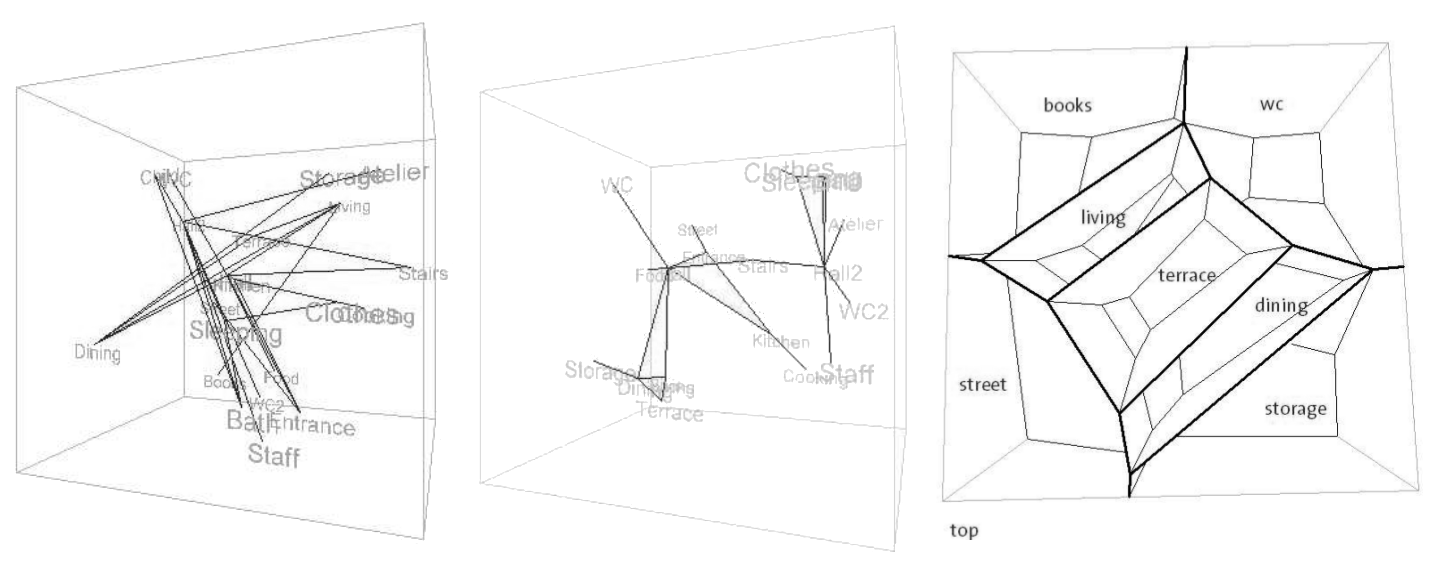
\includegraphics[width=\textwidth]{./Images/8-StructureVoronoi}
\caption[Voronoi Diagram Space Decomposition]{An example of Voronoi Diagram internal space decomposition \cite{friedrich08}}
\label{VDInternal}
\end{figure}

\subsection{Fractals}

"Fractal Geometry is the study of mathematical shapes that display a cascade of never-ending, self-similar, meandering\footnote{\emph{Meander}: to follow a winding or intricate course \cite{merriam03}} detail as one observes them more closely\ldots Fractal geometry is a rare example of technology that can reach into the core of design composition" \cite{bovill96}.

Originated by Benoit B. Mandelbrot in 1975 \cite{fasoulaki08}, the term \emph{fractals} defines a mathematical rule to produce geometrical shapes that are self-similar\footnote{Reduced copy of the whole}. A fractal is produced by defining an initiator shape and a rule that replaces this shape with a smaller set of copies of the original shape, such as a symmetrical combination of two copies of the original shape. The process goes on in recursion and repetition with virtually no limit to the number of iterations. Examples of this process are: the Koch curve (Fig. \ref{KochCurve}), Sierpinski Gasket, Contor Sets and Julia Sets (Fig. \ref{Fractal} \subref{JuliaSets}).

\begin{figure}[htbp]
\centering
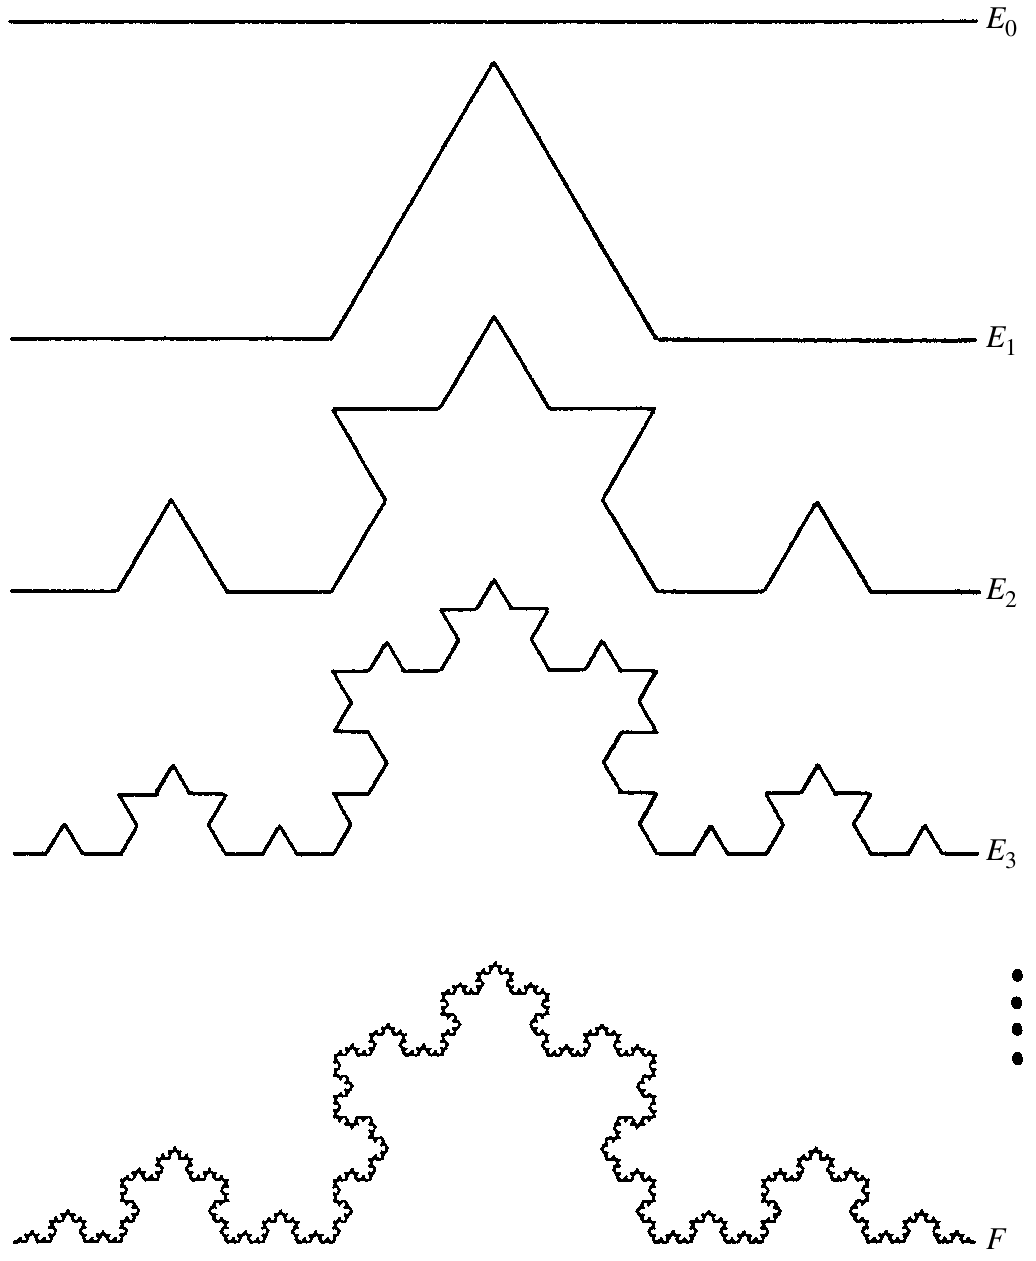
\includegraphics[width=0.8\textwidth]{./Images/9-FractalGeom}
\caption[The Koch Curve]{An example of fractal geometry: The Koch Curve \cite{falconer03}}
\label{KochCurve}
\end{figure}

Fractals are a naturaly occurring phenomenon, such formations of snow flakes, clouds, fern leaves (Fig \ref{Fractal}\subref{Fern}) and coastlines. As mentioned before (\emph{see page} \pageref{NaturalOpt}); the derivation of generative systems from natural formations can be beneficial in optimisational terms of building performance.

\begin{figure}[htbp]
\centering
	\subfloat[Fern Fractal]{{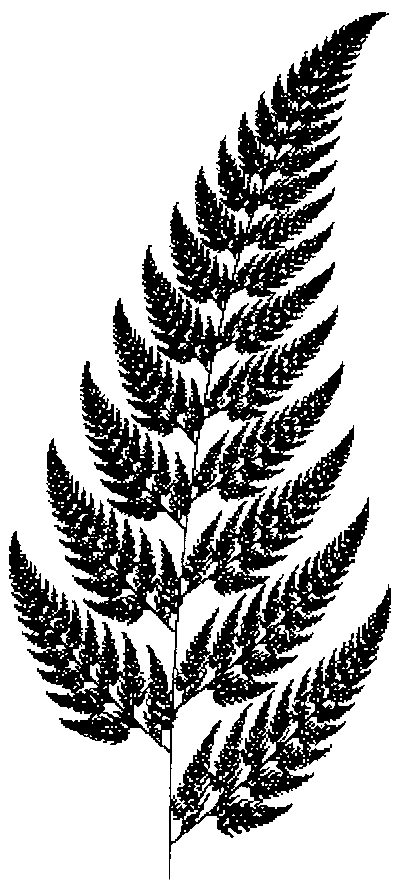
\includegraphics{Images/10-Fern}\label{Fern}}}
	\hspace{2cm}
	\subfloat[Julia Sets]{{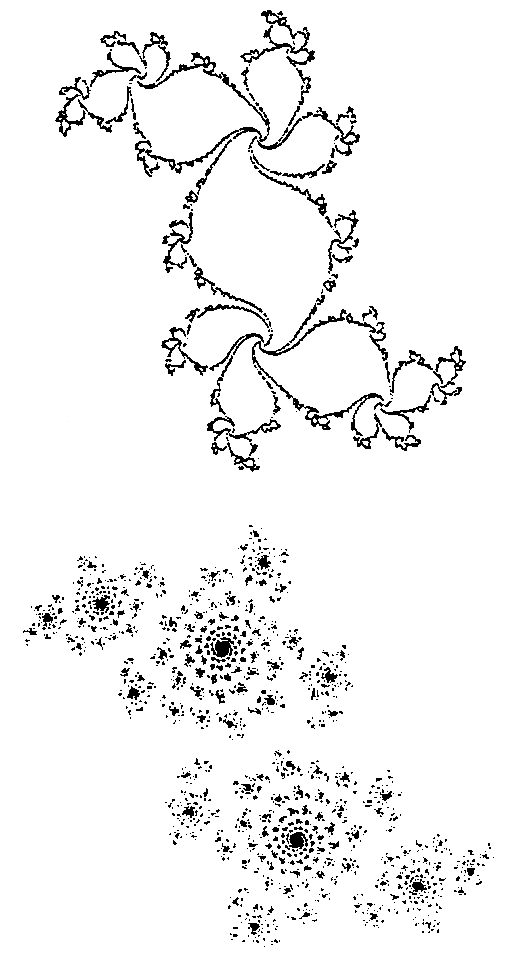
\includegraphics{Images/11-JuliaSets}\label{JuliaSets}}}
	\caption[Fractal Forms]{Fractal Forms \cite{falconer03}}
	\label{Fractal}
\end{figure}

\subsection{Shape Grammars}

A project by George Stiny and James Gips in 1977; shape grammars were intended to be a scientific approach to the language and composition of design. The main goal of shape grammars was to make the design process detached from inidviduals' minds and externalised to something that can be transmitted and modified. A distinctive feature of shape grammars is the visual method of form generation rather than the symbolic or numerical.

As with cellular automata and fractals; the process of generation with shape grammars starts with an initial shape, and is transformed through a given rule. Rules in shape grammars take the form of $A \rightarrow B$. Whenever a shape matching the left side of the rule ($A$) occurs, the rule is applied (Fig. \ref{ShapeGrammarsRule}). As described in a previous section (\ref{AlgoGeoModel}), the type of transformation applied to the shape can addition, subtraction, rotation\ldots etc. 

\begin{figure}[htbp]
\centering
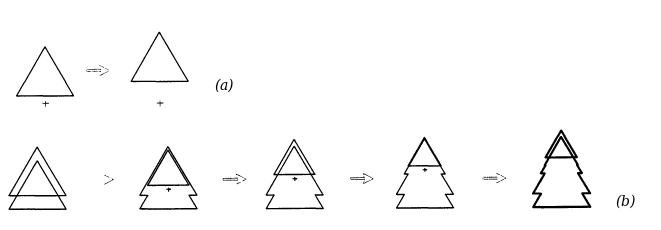
\includegraphics[width=\textwidth]{./Images/12-ShapeGrammarsRule}
\caption[Shape Grammars Rule]{A Shape Grammars Rule: \emph{(a) rule, (b) transformation} \cite{arida04}}
\label{ShapeGrammarsRule}
\end{figure}

Shape grammars also have the ability to apply the rules to emergent shapes; not predefined in the grammar. Shape grammars can be used as a synthezier of shapes be generation, or as an analysis tool of complex shapes; decomposing them into simple ones. Among the many real world applications of shape grammars, a relatively new one was described by D. Shelden \cite{shelden02}; which was during the preparation of contract documents of the \emph{Experience Music} project. The case was the subdivision of a cladded surface for fabrication of the cladding sheets. The surface was divided using a shape grammar rule, but upon receiving the requirements of the fabricator which were smaller sheets; a different rule was used to subdivide the surface (Fig. \ref{SubdivisionSG} -- \ref{SubdFab}).

\begin{figure}[htbp]
\centering
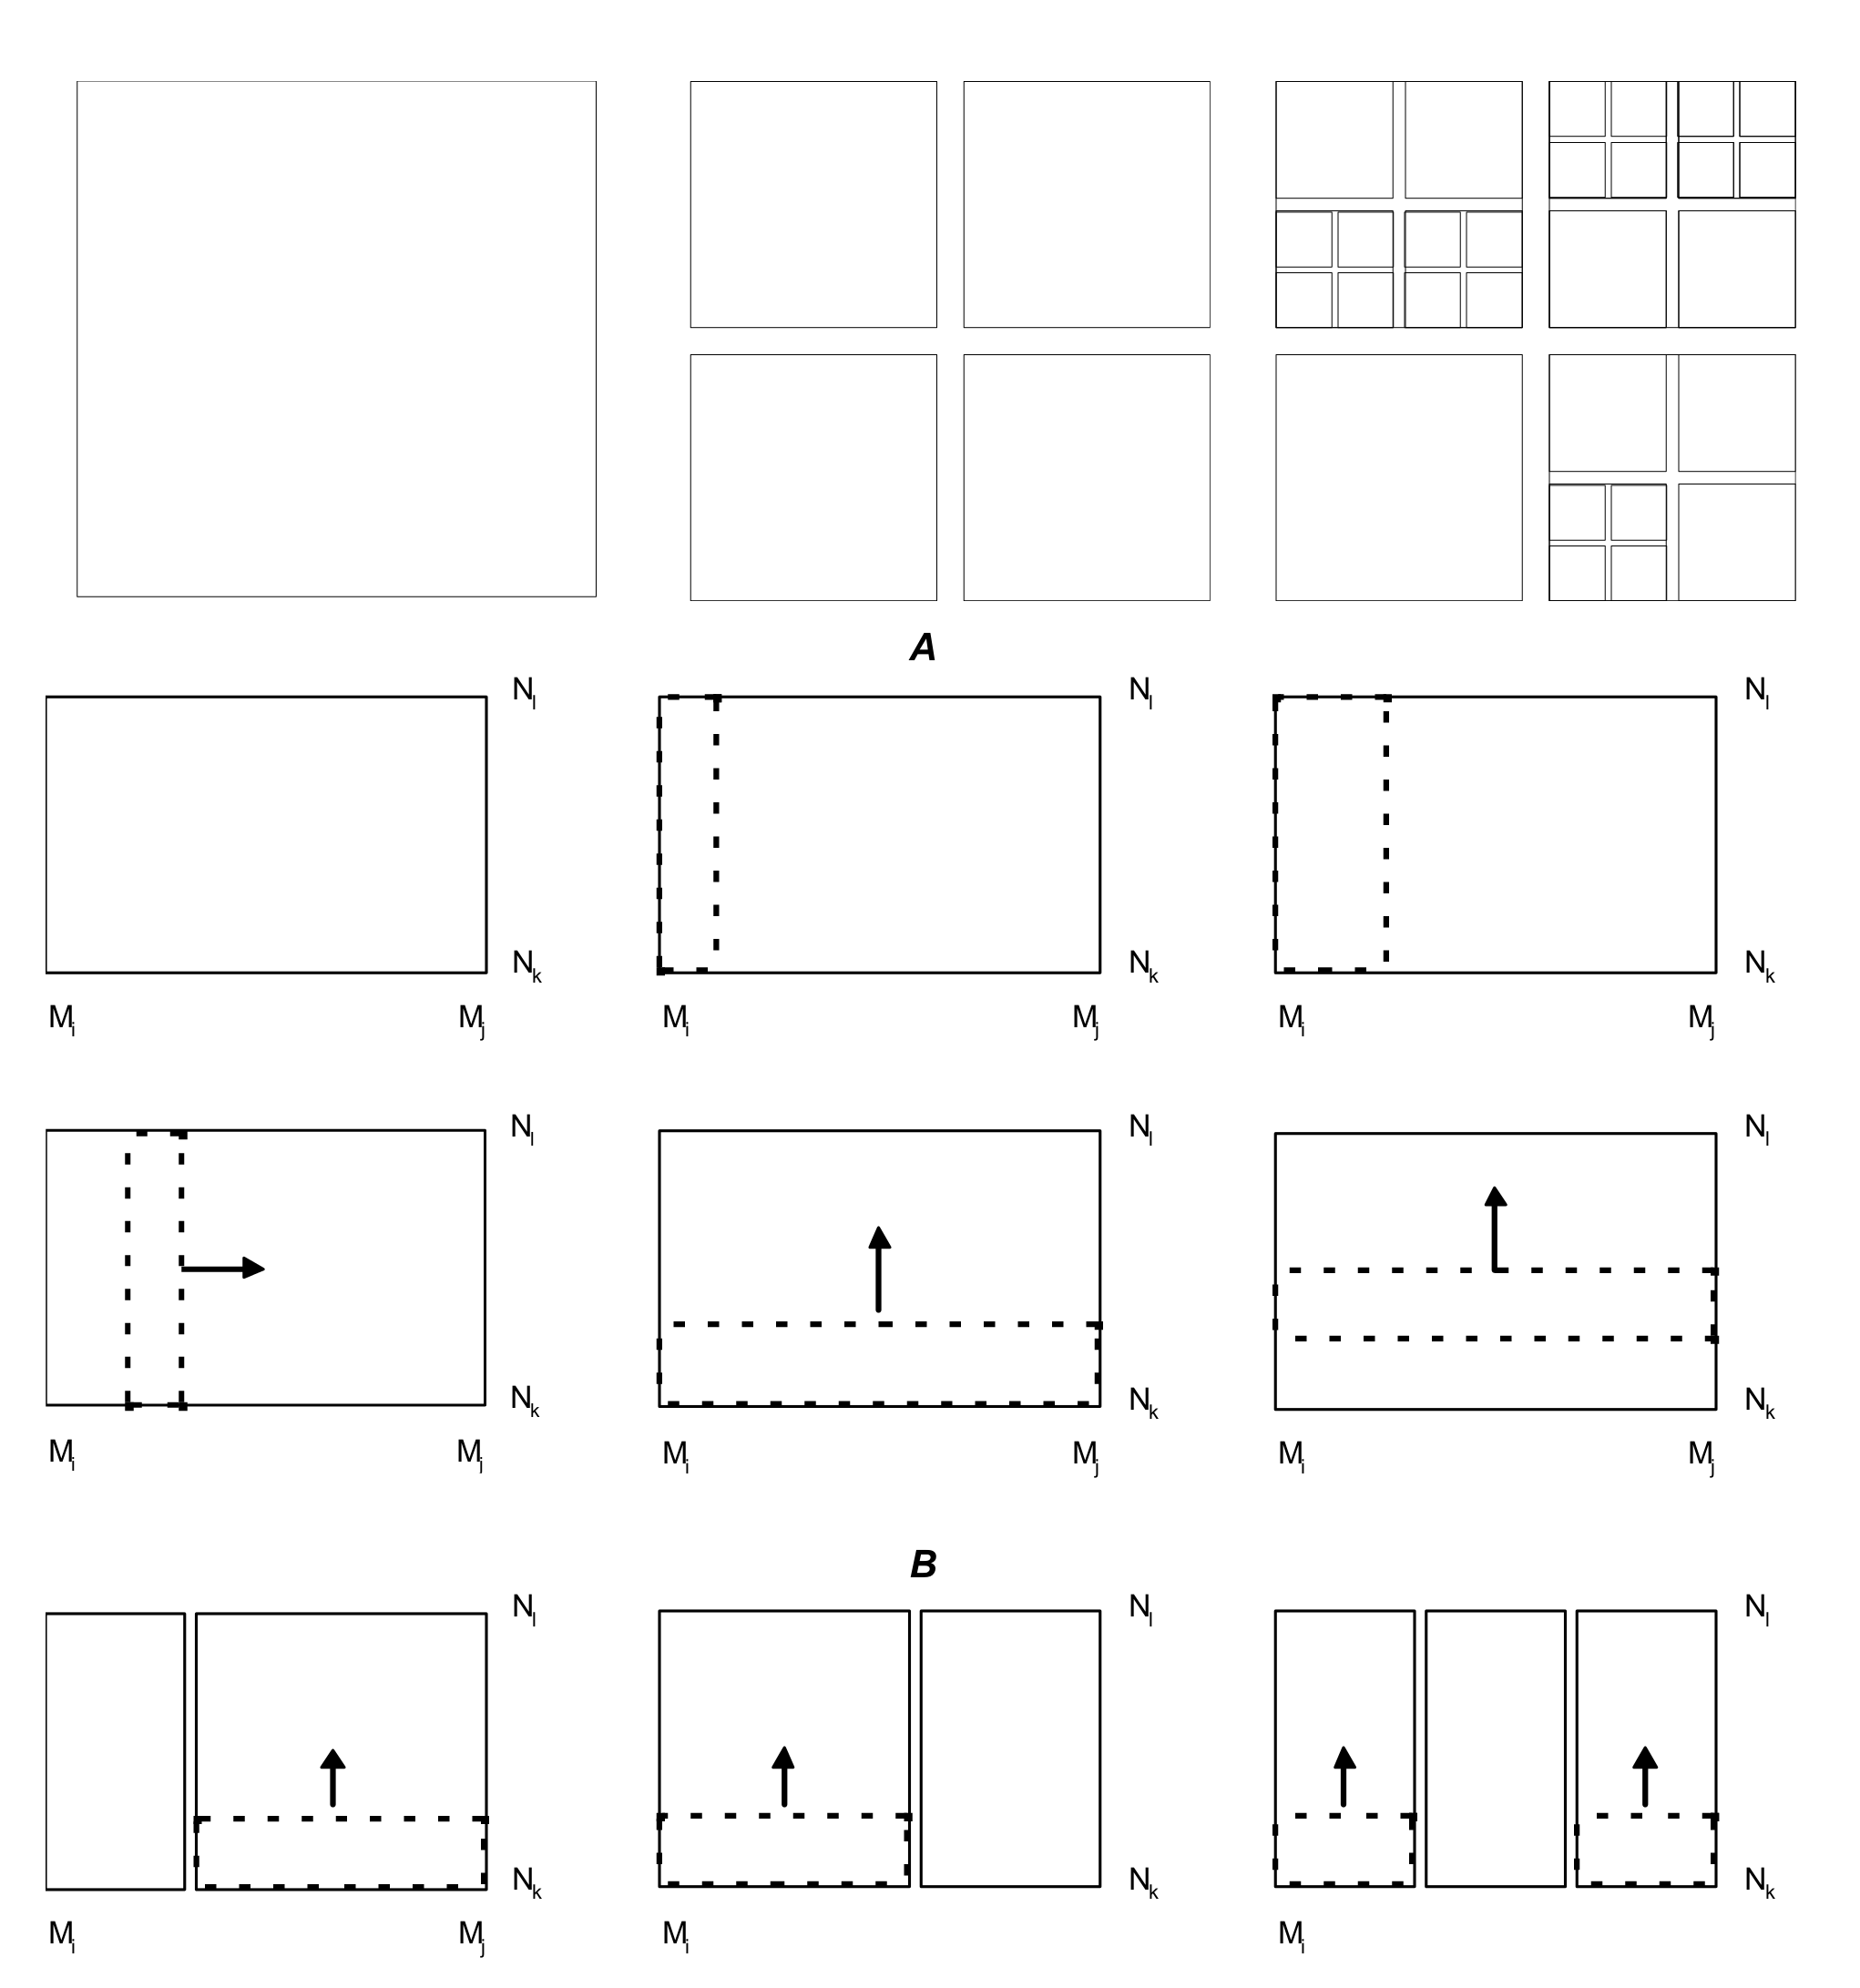
\includegraphics[width=0.5\textwidth]{./Images/13-SubdivisionRule}
\caption[Shape Grammar Subdivision]{The subdivision of a surface by shape grammars for fabrication of the sheets \cite{shelden02}}
\label{SubdivisionSG}
\end{figure}

\begin{figure}[htbp]
\centering
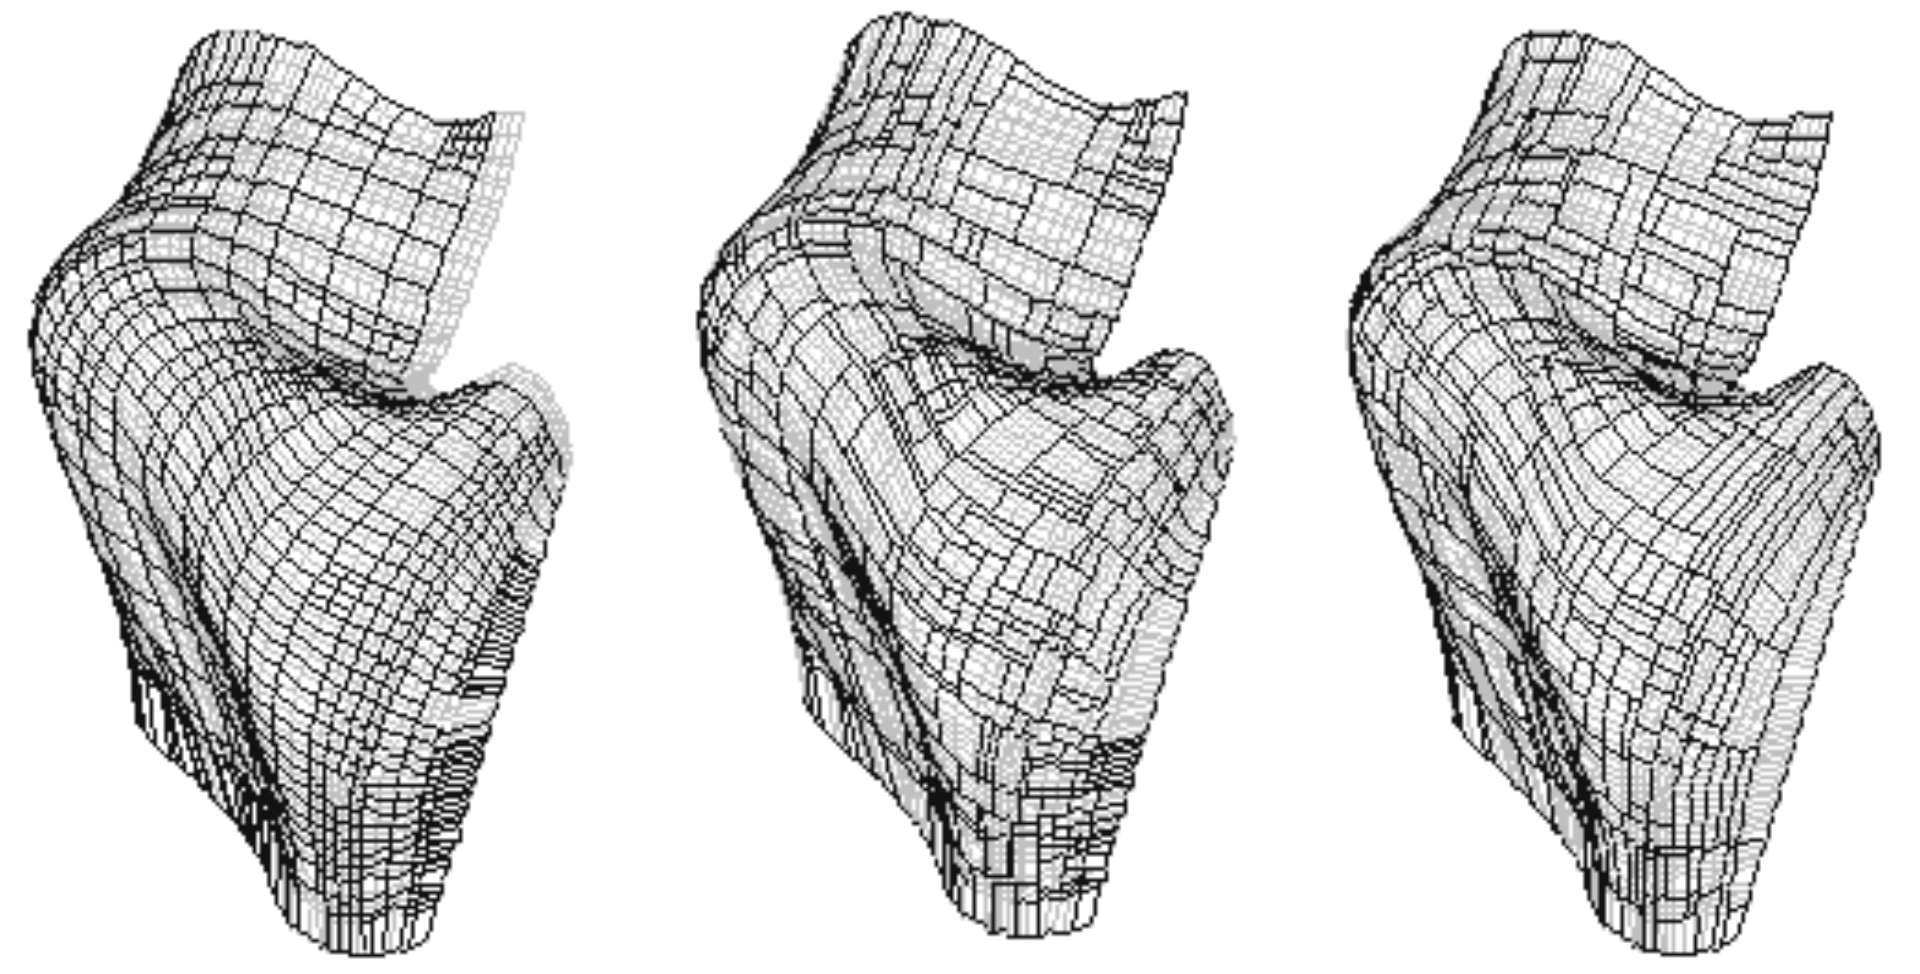
\includegraphics[width=\textwidth]{./Images/14-SurfaceFabrication}
\caption[Fabrication Surface Subdivision]{The subdivision of building envelope for fabricaiton \cite{shelden02}}
\label{SubdFab}
\end{figure}

\subsection{L-Systems}

